\documentclass[10pt,
%superscriptaddress,
%groupedaddress,
%unsortedaddress,
%runinaddress,
%frontmatterverbose, 
%preprint,
%preprintnumbers,
%nofootinbib,
%nobibnotes,
%bibnotes,
 amsmath,amssymb,
 aps,prb, twocolumn
]{revtex4-2}

% Graphics and math
\usepackage{graphicx}
\usepackage{bm}
\usepackage{dcolumn}
\usepackage{physics}
\usepackage{soul}
\usepackage{dsfont}
\usepackage{xcolor} % for more colors
\usepackage{ulem,lipsum}
\usepackage[percent]{overpic} % for captions
% Subfigures (compatible with REVTeX)
\usepackage[caption=false]{subfig}  
%\captionsetup[subfloat]{position=top,justification=raggedright,singlelinecheck=false}
% Hyperlinks (must come last)
\usepackage[colorlinks=true,allcolors=blue]{hyperref}

\newcommand{\id}{\mathds{1}}
\newcommand\sj[1]{ {\color{cyan} #1} } 
\newcommand\del[1]{ {\color{orange} #1} } 
\newcommand\jm[1]{ {\color{magenta} #1} } 
\definecolor{mediumgreen}{HTML}{228B22} % forest green-ish
\newcommand\oz[1]{ {\color{mediumgreen} #1} } 


\begin{document}


\title{Reflectometry Beyond Weak Measurement}

\author{Santiago Salazar Jaramillo}
\email{santiago.salazar-jaramillo@uni-konstanz.de}

\author{Jeff Maki}
% \email{jeffrey.maki@uni-konstanz.de}

\author{Oded Zilberberg}
% \email{oded.zilberberg@uni-konstanz.de}

\affiliation{Department of Physics, University of Konstanz, 78464 Konstanz, Germany}

\date{\today}

\begin{abstract}
    We develop a minimal model of a single measurement event between a qubit and a detector particle...
\end{abstract}

\maketitle

\section{Introduction}\label{sect:intro}

One scheme for describing measurements in quantum mechanics is the von Neumann measurement kick (VN)~\cite{vonNeumann1932}. In this paradigm, the system and the detector are treated as two quantum systems interacting with one another for a short duration. This momentary interaction entangles the system and detector, correlating an observable in the detector to the state of the system. This interaction is often assumed to satisfy quantum non-demolition, which minimizes the uncertainty in subsequent measurements of the system observable~\cite{braginskyNondemolition1996}. The VN paradigm leads to the notion of weak measurements, and can be used to study a variety of phenomena such as continuous monitoring~\cite{wisemanQuantumTrajectorie1996,
bauerRepeatedNonDemolition2013}, weak values~\cite{aharonov1988, alonso2005}, coherent transport~\cite{zilberbergCotunneling2014, KehreinCTAP2011,zilberbergCTAP2019} and the quantum Zeno effect~\cite{doggenzeno2023}.
 
Modern mesoscopic detectors can realize the VN scheme with high
fidelity~\cite{field1993, pilgramEfficiencyMesoscopic2002,
boissonneaultDispersiveNondemo2009}. One commonly used detector is the quantum point contact (QPC), which is used for noninvasive charge readout of quantum dots by correlating the current flowing through a constriction to the occupation of the quantum dot ~\cite{reillyFastSinglechargeSensing2007, peterssonOneElectron2010, vandersypenDetectionElectron2004}. Physically, both QPC and quantum dots are constructed from a 2D electron gas at the interface of a semiconductor heterojunction~\cite{vanhouten1996}, as shown in Fig.~
\ref{fig:fig1}(a). Due to their simplicity QPCs are a paradigmatic example of VN measurements, and have been used to investigate continuous monitoring and the quantum Zeno effect~\cite{gurvitz1996, gurvitzQuantumDescriptionClassical2003,
korotkovMeasurementDoubleDot1999}, and weak values \cite{zilberbergSensingAmplification2011, romito2012}.

Quantum point contacts are most well suited for quantum dots with Rabi
oscillations slower than the individual kick times, as faster oscillations cause charge fluctuations in the quantum dots and impact the signal-to-noise ratio~\cite{reillyFastSinglechargeSensing2007,kumbhakarShotNoise2025}. To obtain a good signal-to-noise ratio for faster oscillations, it is necessary to increase the QPC bias voltage. This however, can lead to drastic measurement backaction effects~\cite{fergusonPopulationSwitch2023}. An alternative to increasing the voltage is to develop a measurement protocol that includes the charge fluctuations that can occur when the Rabi frequency is comparable to the measurement kick. This necessitates a description of the VN measurement kick beyond the standard non-demolition limit.

Treatments relaxing the non-demolition condition remain focused on current based measurements~\cite{engelMeasurementEfficiency2004, svastitsReadoutSweetSpots2026,
molmerQuantumNondemo2022, vaartjesMaximizingNondemo2026,
youngInelasticBackaction2010}. Such treatments yield semiclassical and ensemble-averaged rate equations, and do not provide information about the measurement backaction from a single measurement kick. For this reason, these approaches are not capable of understanding the entanglement induced by the measurement kick.
 
In this work, we present a microscopic model for a single measurement kick in a QPC as a single spin-polarized electron Gaussian wavepacket interacting with a two-level quantum dot, Fig.~\ref{fig:fig1}(b). This model allows us to systematically relax the non-demolition assumption, and capture the full quantum nature of the measurement kick, including entanglement. Depending on the Rabi frequency of the quantum dot and the group velocity of the electronic wavepacket, we find three dynamical regimes, characterized by distinct entanglement entropies. When the Rabi frequency of the quantum dot is slow compared to the group velocity of the electron, we recover the standard non-demolition limit of weak measurements. 

In the opposite regime of fast Rabi oscillations, the system and detector are effectively decoupled. In the intermediate regime, where non-demolition fails, an inelastic scattering channel opens. Our results suggest that protocols beyond non-demolition may be desirable rather than merely tolerable, especially for fast-driven quantum dots which are commonly employed in semiconductor-based quantum computing~\cite{lossQuantumComputation1998, scappucciGermaniumQuantum2021}.

This paper is structured as follows. Section~\ref{sect:model} presents the model and its decoupled properties. Section~\ref{sect:results} defines the unitary entanglement protocol and reports numerical exact diagonalization results, supplemented with a perturbation theory analysis of the three regimes. Finally, Section~\ref{sect:disc_outlook} discusses the results in the context of current-based treatments of inelastic backaction and of photon-assisted and Fano resonances.

\section{Microscopic Hamiltonian for coupled detector and qubit}\label{sect:model}

The Hamiltonian for the total system comprised of the quantum double dot [i.e.\ the qubit] and QPC is
\begin{equation}\label{eq:qpc_dd_H}
    \hat{H} = \hat{H}_S + \hat{H}_D + \hat{H}_I \,,
\end{equation}
as shown in Fig.~\ref{fig:fig1}(a). The Hamiltonian for the qubit is given by
\begin{equation}\label{eq:H_qubit}
    \hat{H}_S = -\Omega \big(\ket{0}\bra{1} + \ket{1}\bra{0}\big) \,,
\end{equation}
and describes Rabi oscillations at frequency $\Omega$ between the two states of the qubit $|0\rangle$ and $|1\rangle$.
Diagonalizing Eq.~\eqref{eq:H_qubit} yields the symmetric and antisymmetric eigenstates \mbox{$|\pm\rangle = \frac{1}{\sqrt{2}}(\ket{0}\pm\ket{1})$} with corresponding eigenenergies $\epsilon_\pm = \mp \Omega$.

The Hamiltonian for the QPC detector is modelled using a one-dimensional tight binding chain
\begin{equation}\label{eq:H_detector}
    \hat{H}_D = -t \sum_{j=1}^N\left( \hat{c}^{\dagger}_{j+1}\hat{c}^{\phantom{\dagger}}_{j} + \hat{c}^{\dagger}_{j}\hat{c}^{\phantom{\dagger}}_{j+1} \right) \,,
\end{equation}
where \mbox{$\hat{c}_j^{(\dagger)}$} annihilates (creates) an electron in the QPC at lattice site 
\mbox{$j$} and 
\mbox{$t$} denotes the nearest-neighbor hopping amplitude. Imposing open boundary conditions on the \mbox{$N$}-site chain produces standing-wave modes with dimensionless wavenumber \mbox{$ka = n\pi/(N+1)$} for integer mode indices \mbox{$n$} and lattice spacing \mbox{$a$}.
In the non-interacting limit, the QPC has a dispersion relation $E(k) = - 2 t \cos(ka)$.
The total energy in the non-interacting limit can be viewed as a set of two bands, depending on whether the qubit is in a symmetric or anti-symmetric state \mbox{$E_\nu(k) = E(k)+\epsilon_\nu$}, see Fig.~\ref{fig:fig1}(b).

The interaction between the QPC and the qubit modifies the hopping of the electron between sites $j=b$ and $j=b+1$ depending on the  occupation of the qubit in state $|1\rangle$
\begin{equation}\label{eq:H_int}
    \hat{H}_I = \frac{g}{2}\hat{c}^{\dagger}_{b+1}\hat{c}^{\phantom{\dagger}}_{b} \otimes \ket{1}\bra{1} + \text{h.c.} \,,
\end{equation}
where $g/2$ measures the reduction of the current.
This local potential barrier correlates the spatial transmission of QPC particles with the internal state of the double dot.

\begin{figure}
    \centering
    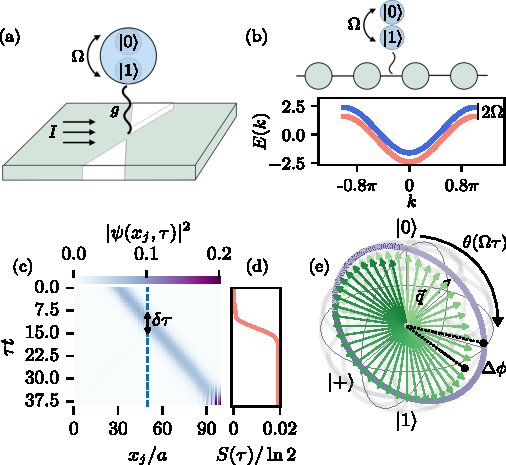
\includegraphics[width=1.0\linewidth]{Figures/fig1.pdf}
    \caption{(a) Schematic of the measurement of a qubit by a QPC. The QPC is a two-dimensional electron gas in the presence of a constriction, through which current $I$ flows due to a voltage bias. The qubit is a double quantum dot with states \mbox{$|0 \ (1)\rangle$} undergoing Rabi oscillations at a frequency \mbox{$\Omega$}, which is capacitively coupled to the QPC current with strength $g$. (b) Schematic of the Hamiltonian Eq.~\eqref{eq:qpc_dd_H} with the eigenenergies of Eq.~\eqref{eq:H_qubit} and Eq.~\eqref{eq:H_detector}  of the total system \mbox{$E_{\nu}(k)$}. (c)-(d) Example of a Von Neumann measurement kick for \sj{\mbox{$g=$}}, \sj{\mbox{$k_0 = $}}, \sj{\mbox{$\Omega = $}}. (c) The QPC occupation as a function of time $\tau t$.  the location \mbox{$x_b$} of the bond site as the dashed line. (d) The dynamics of the qubit in the absence of  (blue dots) and presence of  (green arrows) measurement, where darker colors indicate a later points in time. The black arrow represents the qubit's state when the wavepacket arrives at the bond as detailed in Appendix \ref{app:numerical_setup}.}
    \label{fig:fig1}
\end{figure}

\section{Results}\label{sect:results}
We begin by outlining the initial state preparation and characterizing the unitary time evolution of the electronic wavepacket in the QPC Next, we analyze the resulting measurement backaction on the qubit across different dynamical regimes. Finally, we formulate a perturbative inelastic scattering framework to explain the enhanced measurement efficiency observed at resonance.

\subsection{Flying Detector Protocol and Unitary Dynamics}\label{sect:protocol}
Prior to the measurement event, the injected particle is spatially separated from the qubit. Hence, we initialize the system in the product state
\begin{equation}\label{eq:initial_state}
    \ket{\Psi} = \ket{\psi}\otimes\left(\cos{\frac{\theta_0}{2}}\ket{0}+\sin{\frac{\theta_0}{2}}e^{i\phi_0}\ket{1}\right) \,,
\end{equation}
where the qubit is paramaterized by initial azimuthal and polar Bloch angles $\theta_0$ and $\phi_0$, while the QPC particle occupies a traveling Gaussian wavepacket
\begin{equation}\label{eq:gauss_wavepacket}
    \ket{\psi} = \left(\frac{1}{\pi \Delta_0^2}\right)^{1 / 4} \sum_{j=1}^N e^{-\frac{1}{2 \Delta_0^2}\left(x_j-x_c\right)^2+i k_0\left(x_j-x_c\right)} \hat{c}_j^{\dagger}|\text{vac}\rangle \,,
\end{equation}
with chain coordinates $x_j=ja$, initial wavepacket center $x_c$, and QPC vacuum $|\text{vac}\rangle$. The initial group velocity $v_g(k_0) = 2at\sin(ak_0)$ depends on the initial wavenumber of the wavepacket, \mbox{$k_0$} which is microscopically related to the bias voltage across the QPC. We restrict the central wavenumber to $k_0 > a/\Delta$, so that the initial state contains only right-moving modes and follows a well-defined semiclassical trajectory without reflecting at the boundary at \mbox{$j=1$}.

Comparing the backaction across various injection momenta \mbox{$k_0$} requires a fixed qubit state at the onset of the interactions. This is done by fixing the Bloch angles at a time \mbox{$\tau^* = (x_b - x_c)/v_g(k_0)$}, which is when the Gaussian wavepacket is centered at the bond according to Ehrenfest's theorem. The angle \mbox{$\phi$} does not change under \mbox{$\hat{H}_S$} and so \mbox{$\phi_0$} can be set arbitrarily. The azimuthal Bloch angle \mbox{$\theta$} undergoes Rabi oscillations. We choose \mbox{$\theta_0$} in such a way that the azimuthal angle at time \mbox{$\tau^*$} is given by \mbox{$\theta_M$}. We avoid states at the poles ($\theta_M\neq 0, \pi$) as they represent fully classical states. Otherwise,  different choices of \mbox{$\theta_M$} only renormalize the measurement strength and do not affect the qualitative behavior discussed below [see Appendix~\ref{app:numerical_setup} for more details].

Given the initial state, we solve the unitary time evolution by exact diagonalization of Eq.~\eqref{eq:qpc_dd_H} on a chain of $N=100$ sites [see Appendix~\ref{app:numerical_setup}]. We work in dimensionless units, scaling energies by the hopping amplitude $t$ and distances by the lattice spacing $a$. The interaction strength is set to be $g=0.1t$ and initial width of the Gaussian wavepacket $\Delta_0=7a$ for the remainder of this work. 

An example of the time evolution of the Gaussian wavepacket is shown in Fig.~\ref{fig:fig1}(c). The wavepacket propagates freely until it reaches the bond at time $\tau^*$ with a broadened spatial width $\Delta(k_0)$. It crosses the qubit after a finite measurement time $\delta \tau = \Delta(k_0)/v_g(k_0)$ and afterwards continues its free evolution. We truncate the simulation once the wavepacket center reaches the final lattice site in order to avoid finite-size affects due to reflection at the boundaries.

The dynamics shown in Fig.~\ref{fig:fig1}(c) implement a single VN measurement kick of strength $g\delta \tau$~\cite{vonNeumann1932,svensson2013, siddiqi2024, tamir013}. The central momentum fixes the measurement strength, and is at a minimum when the group velocity is maximum [ \mbox{$k_0 \approx \pi /2$}]. During this time, the wavevepacket becomes entangled with the qubit's density in state \mbox{$\ket{1}$}. We quantify this bipartite entanglement by the von Neumann entropy $S=-\Tr(\hat{\rho}_q\ln\hat{\rho}_q)$, with $\hat{\rho}_q$ the reduced density matrix of the qubit shown in Figs.~\ref{fig:fig1}(d-e). 

Fig.~\ref{fig:fig1}(d) shows the entanglement entropy of the qubit as a function of time for the dynamics in Fig.~\ref{fig:fig1}(c).
The entropy only grows during the measurement time window, where the wavepacket has significant overlap with the qubit. After this time, the QPC and qubit decouple and the entropy saturates. The plateau value of $S$ characterizes the measurement event, and is the focus of our analysis throughout. 

% For horizontal  fig 2 -----
\begin{figure*}
  \centering
    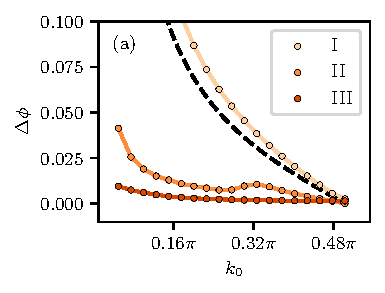
\includegraphics[width=0.325\linewidth]{Figures/phase_v_k0.pdf}
    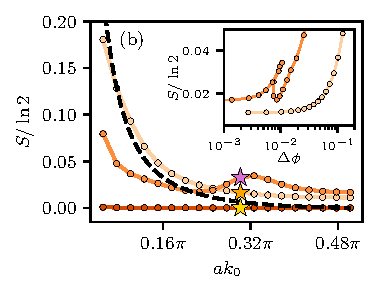
\includegraphics[width=0.325\linewidth]{Figures/entropy_v_k0.pdf}
    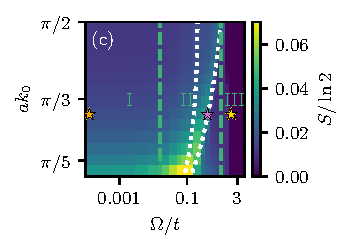
\includegraphics[width=0.325\linewidth]{Figures/entropy_vs_K0_and_om.pdf}
  \caption{Measurement induced backaction and entanglement on the qubit, with the three observed regimes labeled as I) slow qubit with \mbox{$\Omega/t = 10^{-4}$}, II coherent (\mbox{$\Omega/t = 0.4 $}) and III Floquet (\mbox{$\Omega/t = 2.0 $}). The von Neumann entropy $S$ is normalized by \mbox{$\ln{2}$}. (a)-(b) Phase shift and entanglement as a function of \mbox{$k_0$} for three different Rabi frequencies. ED results are shown as red dots and the dashed lines were obtained with Eq.~\eqref{eq:phase_gain} and Eq.~\eqref{eq:entropy_gain}. The inset in (b) plots the entanglement entropy against measurement backaction for regimes I and II, where points close to $k_0 = \pi/3$ are highlighted as blue diamond. (c) Color map for the entropy as a function of \mbox{$k_0$} and \mbox{$\Omega$}, the green dashed lines indicate the boundaries between regimes set by Eq.~\eqref{eq:entropy_bounds} and the white dotted lines are the bound in Eq.~\eqref{eq:k0_bounds}. The points marked with star markers correspond to each other in both figures.}\label{fig:fig2}
\end{figure*}

In addition to the entropy, the reduced density matrix also gives the measurement backaction on the qubit, which is characterized by the vector $\vec{q}$ on the Bloch sphere. This is shown in Fig.~\ref{fig:fig1}(e) which compares the trajectory of \mbox{$q$} in the presence of measurements against free Rabi oscillations. Initially, $\vec{q}$ follows the same orbit as the free case. After entanglement with the wavepacket, $\vec{q}$ still undergoes Rabi oscillations at the same frequency, but the plane of rotation is shifted by a polar angle \mbox{$\Delta \phi$}, which corresponds to a phase gain [see Eq.~\eqref{eq:initial_state}]. After the interaction, the measured $\vec{q}$ continues following its new orbit. In addition, the magnitude of the Bloch vector is no longer unity, due to entanglement with the detector, see Fig.~\ref{fig:fig1}(d). Therefore, the backaction on the qubit is characterized by \mbox{$\Delta \phi$} and the plateaued entropy, while the Rabi frequency remains unchanged.

These two quantities, depend strongly on the wavenumber \mbox{$k_0$}. In Fig.~\ref{fig:fig2}(a-b) we examine how the phase gain and the entanglement entropy change as a function of \mbox{$k_0$} for three different $\Omega \delta\tau$. We observe three distinct regimes. 

In the \textit{slow-qubit regime} ($\Omega\delta\tau\ll1$), the \mbox{$g \delta \tau$} alone determines the measurement backaction. The qubit is approximately stationary during this time, so the wavepacket effectively scatters off of a static barrier. In this regime both $\Delta\phi$ and $S$ decrease monotonically with $k_0$, since faster wavepackets spend less time at the measurement bond. The qualitative behavior can be understood using a toy model that that realizes the standard non-demolition VN measurement~\cite{braginskyNondemolition1996} that couples the scattering phase in the QPC \cite{buttikerTunnelingTime1982, aleinerOrthogonalityCatastrophe1997,sankarDetectorTuned2024} to the density at the double dot to  [see Appendix~\ref{app:derivation_backaction} for more details]. In this model, the qubit's phase gain
\begin{equation}\label{eq:phase_gain}
    \Delta \phi (k_0) = \frac{g}{2t} \cot{k_0 a} +\mathcal{O}\left(g^2\right) \,,
\end{equation}
appears as the first order correction to its reduced density matrix. The second order correction yields the entropy \mbox{$S(k_0) = -\sum_{n=\pm}\lambda_n \ln{\lambda_n}$}. With the eigenvalues \mbox{$\lambda_n = \frac{1\pm \abs{q}}{2}$} depending on $\abs{q} = \sqrt{\sin^2\theta_M R^2 + \cos\theta^2_M}$ in terms of the dephasing factor
\begin{align}\label{eq:entropy_gain}
    R(k_0) = & \exp\left\{\frac{1}{4 t^2} \left( \cot^2(k_0 a) + \frac{a^2 [1+3\cot^3 (k_0a)]}{2\Delta(k_0)^2 \sin^2(k_0a)} \right)\right\} \nonumber \\ & + \mathcal{O}(g^3).
\end{align}
 Both analytic predictions, shown in Fig.~\ref{fig:fig2}(a)-(b) as black dashed lines. \sj{The commutators for the toy model explicitly show all terms that break the non-demolition condition are linear in \mbox{$\Omega$}, hence non-demolition requires an effectively static qubit during \mbox{{$\delta\tau$}}.}

The opposite \textit{fast-qubit regime} ($\Omega\delta\tau\gg1$), suppresses the backaction altogether. This is intuitive as the qubit completes many Rabi cycles while the wavepacket crosses the bond. The detector hence samples only the time-averaged qubit density, which acts as a static potential barrier and carries away no information. This results in the decoupling of the detector and qubit, as is reflected in the ED results labeled as III, where both \mbox{$\Delta \phi$} and \mbox{$S$} vanish.

The \textit{coherent regime} (labeled as II) is defined when $\Omega\delta\tau \approx 1$, thus breaking non-demolition [Appendix~\ref{app:derivation_backaction}]. In this regime both $\Delta\phi$ and $S$ exhibit a peak at around $k_0 \approx 0.3\pi$. Near the peak, the entanglement entropy for the coherent regime surpasses the corresponding slow-qubit curve. This suggests a higher measurement efficiency, as confirmed by the inset of Fig.~\ref{fig:fig2}(b). Here, the entropy is plotted against the phase gain. The curve corresponding to the coherent regime is consistently above the slow qubit curve, indicating that higher entanglement is achieved for the same measurement backaction.

We confirm the distinction between the three regimes by exploring the entanglement entropy across the full parameter space, shown in Fig.~\ref{fig:fig2}(c). The slow-qubit entropy [I] is independent of $\Omega$ and grows toward small $k_0$, due to the increase in \mbox{$\delta \tau$}. The fast-qubit entropy [III] vanishes globally. The coherent regime [II] instead hosts a distinct band of enhanced entropy. Near $k_0 = \pi/2$, the band is confined to Rabi frequencies close to $t$, and it broadens as $k_0$ decreases and the measurement time grows. This feature is not captured by either slow (non demolition) or fast-qubit limits. As we discuss below, the origin of this feature is due to an inelastic scattering channel that only becomes available in the coherent regime.

\subsection{Inelastic Scattering and Entanglement}\label{sect:entanglement}

The mechanism behind the resonant band can be understood by investigating how interactions lead to a non-trivial superposition of qubit eigenstates. We can identify such processes by calculating the corrections to the eigenstates to first order in \mbox{$g$} [see Appendix~\ref{app:derivation_perturbative}]
\begin{widetext}
\begin{align}
    \ket{\Phi_\nu^{(1)} (k)} = &  \frac{g}{2(N+1)} \frac{\xi(k,k)}{2\epsilon_\nu} \ket{k} \otimes \ket{\bar{\nu}} \nonumber \\
    & +\frac{g}{2(N+1)} \sum_{p \neq k} \ket{p} \otimes \left\{\frac{\xi(k,p)}{-2t(\cos ak - \cos ap)} \ket{\nu} + \frac{\xi(k,p)}{2\epsilon_\nu - 2t(\cos ak - \cos ap)} \ket{\bar{\nu}} \right\}. \label{eq:psi_first_order}
\end{align}
\end{widetext}
In Eq.~\eqref{eq:psi_first_order}, Greek indices label the qubit's quantum number \mbox{$\nu=\pm$} (with \mbox{$\epsilon_\nu=-\nu\Omega$} and \mbox{$\bar{\nu}\neq\nu$} throughout), while \mbox{$\xi(k,p)=\sin(x_b k)\sin\!\big((x_b+a)p\big)+\sin(x_b p)\sin\!\big((x_b+a)k\big)$} is a function of the lattice momenta.

The first term in Eq.~\eqref{eq:psi_first_order} mixes the different the qubit eigenstates at fixed momentum in the QPC. The denominator depends only on the Rabi frequency, and therefore grows without bound as \mbox{$\Omega\rightarrow0$}. This term dominates the slow-qubit regime~[I].
\del{Notwithstanding that growth, the divergence marks the degeneracy of the two
qubit levels rather than strong entanglement \sj{(One sentence giving an intuition then derive in appendix)}.}

In contrast, the second term dominates in the fast qubit regime~[III], and is equivalent to elastic scattering due to an impurity. This term does not couple different qubit states together, and as such does not produce entanglement.

The third term couples eigenstates of the system with different momenta and qubit quantum numbers. This term will produce entanglement entropy, in line with our intuition. This term is strongest when the kinetic energy difference in the detector matches the Rabi frequency, 
\begin{align}\label{eq:resonance_condition}
   \abs{\Delta E(k,p)}= 2 \Omega. 
\end{align}
This resonance condition corresponds to an inelastic scattering process where the detector exchanges energy with the qubit. This process is only possible when the Rabi frequency sits within the bandwidth of the QPC
\begin{align}\label{eq:entropy_bounds}
    \frac{1}{2} \text{min}|\Delta E(k,p)| \leq \Omega \leq t.
\end{align}
These bounds correspond to the vertical green dashed lines in Fig.~\ref{fig:fig3}(c), enclosing regime [II]. 

\sj{This energy based picture from Eq.~\eqref{eq:psi_first_order}, is shown to be complementary to the time-depdendent protocol developed in Section~\ref{sect:protocol}, by restating the bounds in Eq.~\eqref{eq:entropy_bounds} for the wavepacket. The upper bound, is the maximum energy \mbox{$\Delta E_{\text{max}} = E(k_0)-E(0)$} that a wavepacket with $k_0$ is capable of transferring to the qubit. The lower bound is recovered in terms of resolution. For \mbox{$\text{min}|\Delta E(k,p)|$} to involve two distinguishable states, the output wavenumber $p$ has to be outside the wavepacket bandwidth, at least \mbox{$\Delta E_{\text{min}}(k_0,k_0\pm 1/\Delta (k_0)) \approx 2t\sin{k_0 a}/\Delta(k_0) = 1/\delta \tau$}. Therefore, at the wavepacket level, Eq.~\eqref{eq:entropy_bounds} is analogous to
\begin{equation}\label{eq:k0_bounds}
    \frac{1}{2\delta\tau}\leq \Omega\leq t(1-\cos(ak_0)),
\end{equation}
plotted as the dotted white lines in Fig.~\ref{fig:fig2}(c), approximately enclosing the resonant band.}

The resonance conditions for this inelastic scattering channel is tested against the spectrum obtained by ED in Fig.~\ref{fig:fig3}. Figure~\ref{fig:fig3}(a) shows the interacting eigenenergies colored by the projection \mbox{$\Pi_-=\id_{\text{QPC}}\otimes\ket{-}\bra{-}$} onto the anti-symmetric qubit
state. Blue points denotes a qubit state fully in the anti-symmetric sector, while red ones are when the qubit is in the symmetric sector. The white dots represent eigenstates of the system in a maximal superposition of symmetric and antisymmetric sectors. These points coincide with the resonance condition, Eq.~\eqref{eq:resonance_condition}, which we denote by the vertical lines. Note we only show the resonant lines for positive momenta as these resonant lines are symmetric about zero momentum.

Figure~\ref{fig:fig3}(b) shows the entanglement entropy of every eigenvector of the total Hamiltonian $\hat{H}$, obtained from the Schmidt decomposition [cf.\ Appendix~\ref{app:numerical_setup}]. The color corresponds to whether the state lies in the upper or lower energy band. The most entangled eigenstates sit exactly at the same momenta as the hybridized pairs in Figure~\ref{fig:fig3}(a), corresponding to Eq.~\eqref{eq:resonance_condition}. Taken together, Fig.~\ref{fig:fig3} shows that our our perturbation theory analysis is consistent with the exact eigenspectrum of the system, and predicts where the measurement efficiency is maximal.

\begin{figure}
    \centering
    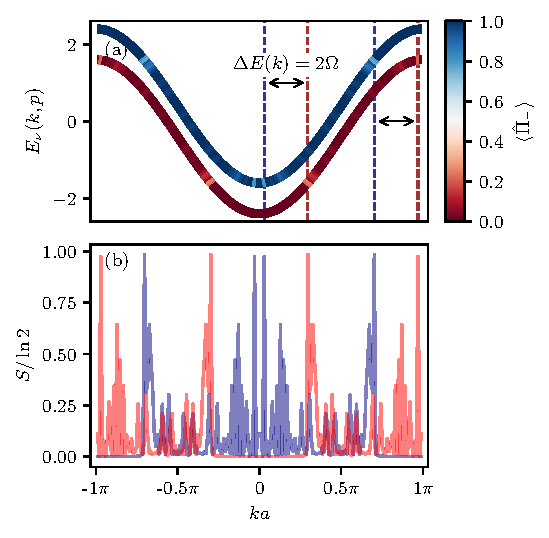
\includegraphics[width=1.0\linewidth]{Figures/band_struct_main.pdf}
    \caption{ED band structure and entanglement for $\Omega = 0.4t$ separated into symmetric (Red), anti-symmetric (Blue) and labeled by momentum k. (a)  Eigenenergies colored by the projection onto the symmetric band of their respective eigenvectors. (b) Entanglement of each eigenvector of $\hat{H}$. The vertical lines indicate the 4 most entangled eigenstates, where dashed/solid lines indicating the resonance.}\label{fig:fig3}
\end{figure}

\section{Discussion and Outlook}\label{sect:disc_outlook}

We have proposed a minimal unitary model of the QPC-qubit measurement process, governed by a Gaussian wavepacket with group velocity determiend by $k_0$, which fixes the duration of the measurement window \mbox{$\delta \tau$}, and the Rabi frequency $\Omega$. The measurement is characterized by the qubit's phase gain $\Delta\phi$ and the entanglement entropy $S$, as shown in Fig.~\ref{fig:fig2}. We observe three distinct regimes the slow-qubit~[I], coherent~[II] and fast-qubit~[III]. 

\sj{As shown in Fig.~\ref{fig:fig2}, Regime [III] does not generate backaction or entanglement as the qubit's fast oscillations average out the coupling potential for the wavepacket, thus decoupling detector and system. Regime [I] represents an effectively static qubit during measurement which guarantees that non-demolition is fulfilled. The static qubit is the underlying assumption behind the rate equation formalism developed in \cite{gurvitz1996, gurvitz1997,gurvitzQuantumDescriptionClassical2003, gurvitzZeno2003}, whose results are consistent with [I] in Fig.~\eqref{fig:fig2}(a)-(b) and represent dephasing due to continuous measurement \cite{korotkovMeasurementDoubleDot1999}. Regime [II] is especially interesting as it exhibits a resonant feature due to coherent exchange of energy between the QPC and the qubit. This is the inelastic scattering channel in Eq.~\eqref{eq:psi_first_order} that becomes available in [II], where the non-demolition assumption is broken. This scattering process is selected by the Gaussian weights in Eq.~\eqref{eq:gauss_wavepacket}, following the bounds in Eq.~\eqref{eq:k0_bounds}. Thus explainig the \mbox{$k_0$} dependence of the resonant feature in Fig.~\eqref{fig:fig2}(c). We stress that at lower $k_0$, our analysis breaks down as the QPC and qubit remain coupled.}

\sj{The inelastic scattering channel in [II] is reminiscent of effects found in a many-body setting such as the Fano mechanism.} Typically, it involves an elastic scattering channel within a continuum interfering with a secondary channel in which the continuum generates an excitation in a discrete state~\cite{kobayashiFano2004, reyesFano2017} (\sj{I suspect I am being sloppy with my fano claim here}). As shown in Fig.~\ref{fig:app_fano}, we observe transmission peaks reminiscent of the Fano interference at larger coupling, suggesting a connection to many-body effects in our two-body setup.

Moreover, inelastic backaction channels have been reported in current-based treatments of the QPC-qubit system ~\cite{ouyangBackaction2010, youngInelasticBackaction2010, chudnovskiyDoubleDot2009}. Our model thus represent a microscopic realization by merging the effects of charge noise and QPC voltage bias in the object of the wavepacket. The former is related to the dwell time of electrons, directly related to \mbox{$\delta \tau$}, while the later is connected to $\Delta_0$ as approximating the momenta available for transport between the left and right leads of a QPC.

Where our model differs is in scope. The microscopic description of a single event under unitary evolution, yields a straightforward metric of information gain and enhanced measurement efficiency as shown in Fig.~\ref{fig:fig2}(b). This is in contrast to thermodynamic entropy extracted from charge measurements via a Maxwell relation~\cite{hartmanDirectEntropy2018, childEntropyMeasurement2022} which is a state function of the probed system. 

\sj{one limitation for our model is that it is restricted to finite chains. This can be seen by noticing that the lower bound in Eq.~\eqref{eq:entropy_fit} vanishes as \mbox{$N\rightarrow\infty$}}. Nevertheless, this limit we argue that the finite tight binding chain \mbox{$\hat{H}_D$} is an appropriate model for the QPC-qubit measurement. It describes the effectively one-dimensional mesoscopic region surrounding the charge sensing constriction of a QPC operating near the first conductance plateau~\cite{vanwees1988, wharam1988, vanhouten1996}, whose extent is set by the phase-coherence length~\cite{bruusManyBodyQuantum2004, tekman1991}. In addition, the entropy regimes and resonant band found in Fig.\ref{fig:fig3}(c) persist as the size of the chain is doubled as shown in Fig.~\ref{fig:app_calibration}, indicating that the regimes and inelastic scattering channel are robust to larger finite chains. \sj{Furthermore, the bridge to the wave packet picture in Eq.~\eqref{eq:k0_bounds} does not depend on $N$, further evidencing the resonant feature is not merely a finite size effect.}

Our results hence provide an information based perspective on the advantages of realxing non-demolition condition. As this involves larger Rabi frequencies, beyond non-demolition measurements may provide a way to fast qubit operation, as required for gate implementation~\cite{wangExperimentalNonadiabatic2016}. Beyond this, our methodology extends to sequences of wavepackets interacting with the qubit in succession, which would allow tests of Leggett-Garg inequalities~\cite{jordan2008}, and to spin and valley degrees of freedom relevant to silicon and germanium quantum dots~\cite{lossQuantumComputation1998, scappucciGermaniumQuantum2021}.
We caution that the latter generalization is not automatic: the constriction couples to charge, so a spin qubit enters only through spin-to-charge conversion or spin-orbit admixture~\cite{borhaniGolovachLoss2006}, and the resonance condition would then involve the charge character of the relevant spin states rather than a bare Zeeman splitting.


\section{Acknowledgments}

This project was funded by (...)

\section{RDM Statement}


\bibliographystyle{apsrev4-2} % APS recommended BibTeX style
\bibliography{qpc}     % Name of your .bib file (witho

\appendix 

\onecolumngrid 

\section{Numerical Methods and Finite Size Effects}\label{app:numerical_setup}

\subsection{Exact Diagonalization Algorithm}

\begin{itemize}
    \item Exact diagonalization.
    \item Exact numerical values used.
    \item Initialization of the independent state and estimation of the final state to avoid finite size effects simulation time with ehrenfest.
    \item Estimation of the phase.
    \item Schmidt decomposition.
    \item Mention finite size
\end{itemize}

As mentioned in the main text, we calculate the time evolution of the composite qubit-QPC system, by performing exact diagonalization on the Hamiltonian Eq.~\eqref{eq:qpc_dd_H}. 

The specific form of the free Hamiltonian and the interaction lends itself to exact diagonalization due to the size of its Hilbert space. The model is effectively a one dimensional system restricted to the 2 particle sector of the full Hilbert space, where there is always exactly one excitation on the QPC and one on the double dot. Therefore,  Eq.~\eqref{eq:qpc_dd_H} is expressed as a $2N$ dimensional matrix (where $N$ is the number of QPC lattice sites) in the computational basis
\begin{align}\label{eq:string_basis}
    \ket{\vec{j}}\otimes \ket{\alpha} = \ket{0\dots \overbrace{1}^{j\text{th site}} \dots0}\otimes\ket{\alpha}
\end{align}
where the notation \mbox{$\ket{\vec{j}}$} represents a size $N$ string of zeros with a single one on site $j$. This is the numerical representation of the abstract vectors \mbox{$\hat{c}_j\ket{\text{vac}}$}. The doubling of the matrix's dimension comes from the qubit's states \mbox{$\ket{\alpha} = \ket{0},\ket{1}$}.

The time evolution is performed by computing the exact eigenvectors and values Eq.~\eqref{eq:qpc_dd_H} and applying the time evolution operator
\begin{align}\label{eq:time_evolution_ed}
    \ket{\Psi{(\tau)}} = e^{i\tau/\hbar \hat{H}}\ket{\Psi (0)},
\end{align}
where the initial state \mbox{$\ket{\Psi (0)}$} (Eq.~\eqref{eq:initial_state}) is transformed to the computed eigenbasis. The evolution is carried out until the wavepacket hits the end of the chain, to avoid reflections. The time of flight is given by Ehrenfest's theorem as
\begin{align}\label{eq:final_time}
    \tau_f = \frac{x_N}{v_g} =  \frac{a N}{2 J \sin{k_0a}}
\end{align}
for a semiclassical wavepacket sharply peaked around $k_0$.

Regarding the initial state of the qubit, as mentioned in Section \ref{sect:protocol}, the initial polar angle $\theta_0$ is dependent on the central wavenumber $k_0$ of the gaussian wavepacket. The reason for this restriction is to guarantee that the qubit is always in the same state when the wavepacket arrives at the bond site and they interact. This allows us to separate the effects of $k_0$ and $\omega$ from those due to a variable qubit occupation. 

Considering a free qubit that passes trough the poles of the Bloch sphere, the initial state is given by the polar angle
\begin{align}\label{eq:qubit_init}
    \theta_0 = - \frac{\theta_M}{2}+\delta\tau \omega
\end{align}
where $\theta_M$ is the free parameter setting the state of the qubit at the time of interaction, and $\Delta \tau$ is the flight time of the wavepacket 
\begin{align}
    \delta \tau = \frac{x_b}{2J\sin(k_0)},
\end{align}
as given by Ehrenfest's theorem.

As mentioned in the main text, the choice of \mbox{$\theta_M$} is largely arbitrary as its net effect is solely to renormalize the strength of the coupling between the QPC and the detector. This is quantified by the transmission through the bond in Fig.~\ref{fig:app_calibration}(a). Here, it is shown that \mbox{$\theta_M$} corresponding to qubits more localized in the \mbox{$\ket{0}$} state have a larger transmission compared to those closer to \mbox{$\ket{1}$}, as the effective potential barrier set by the qubit is lower in this case. We observe that the change in coupling strength roughly follows \mbox{$\tilde{g} \propto g \delta\tau\sin^2\theta_M/2$}. However, we avoid states sitting exactly at the poles of the Bloch sphere \mbox{$\ket{0}$} and \mbox{$\ket{1}$}, as they represent special fully localized states, whereas we are interested in more generic interactions.


The parameters used to create all data in the main text are \mbox{$N=100$}, \mbox{$a=1$}, \mbox{$J=1$}, \mbox{$g=0.1$} \mbox{$k0\in [\pi/6, \pi/2]$}, \mbox{$\Omega\in (10^{-4}, 5)$}, \mbox{$\theta_M=\pi/5$}.



% For horizontal  fig 2 -----
\begin{figure}
  \centering
    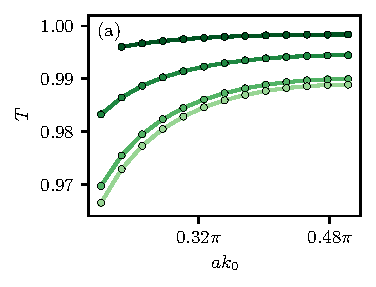
\includegraphics[width=0.325\linewidth]{Figures/qubit_occupation.pdf}
    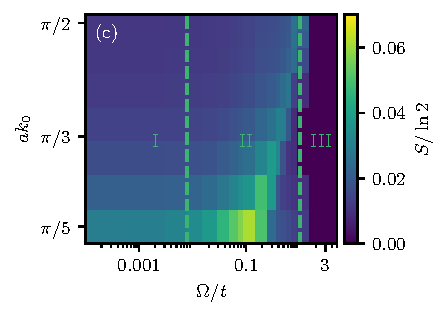
\includegraphics[width=0.325\linewidth]{Figures/finite_size.pdf}
    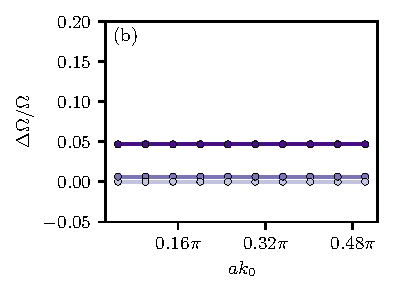
\includegraphics[width=0.325\linewidth]{Figures/change_in_rabi.pdf}
  \caption{Calibration of the exact diagonalization algorithm. (a) Transmission through the bond as a function of \mbox{$a k_0$} for different qubit states  at the time of measurement as given by Eq.~\eqref{eq:qubit_init}. Each color denotes a different angeles \mbox{$\theta_M \in \{0, \pi/5, \pi/2,3\pi/4\}$}, ordered from light green for small values to dark green for large values of \mbox{$\theta_M$}. )(b) Entanglement entropy as a function of $k_0$ and $\Omega$ for a QPC with \mbox{$N=200$} sites. The green dashed lines correspond to the bounds in Eq.~\eqref{eq:entropy_bounds}.(c)  Relative change in Rabi frequency $\Delta \Omega$ as a function of \mbox{$a k_0$} for initial Rabi frequencies \mbox{$\Omega/t = 10^{-3}, 0.4, 2.0$} colored light, medium and dark blue respectively.}\label{fig:app_calibration}
\end{figure}

\subsection{Numerical Estimation of Observables}

\begin{align}\label{eq:app_schmidt_deco}
    \Phi = 
\end{align}

\begin{align}\label{eq:entropy_fit}
    S(k_0) = \text{Include the fitting error here}
\end{align}

\section{Von Neumann's Measurement Scheme}\label{app:derivation_backaction}

The following is a realization of von Neumann's measurement kick \cite{vonNeumann1932}, which captures the physics of the Hamiltonian in Eq.\eqref{eq:qpc_dd_H} for a non-demolition measurement in the slow qubit regime. Throughout this section, we  approximate the detector Hamiltonian $\hat{H}_D$ as an infinite tight-binding chain, and assume our wave packet is sharply peaked around a $k_0$ central wave number. 

First, to have a proper measurement kick, it is necessary that the interaction between detector and observed system commutes with the detector's Hamiltonian \cite{vaartjesMaximizingNondemo2026}, which \mbox{$\hat{H_I}$} fails to do. Therefore one needs to find a suitable replacement. A naive procedure follows von Neumann's original treatment of a free particle by replacing the interaction Hamiltonian with 
\begin{align}
    \hat{h}_I = \frac{g}{2} \hat{K} \otimes \ket{1}\bra{1},
\end{align}
in terms of the crystal momentum $\hat{K}$, where $\hat{K}$ is defined by its action \mbox{$K\ket{k}=ak\ket{k}$} on \mbox{ $\hat{H}_D$}'s eigenfunctions. Given that \mbox{$\ket{k}$} are also eigenstates of the crystal momentum, it immediately commutes with \mbox{ $\hat{H}_D$}. An additional advantage is easy of interpretation. Given that $\hat{K}$ is the generator of translations, the role of \mbox{$\hat{h}_I$} is to shift the center of the wavepacket conditioned on wether the qubit is in state \mbox{$\ket{0}$} or \mbox{$\ket{1}$}. Thus, the qubit's state can be inferred from the observed position of the detector wavepacket. 

However, this choice is only suitable for low-energy states situated near the minimum of the Brillouin zone, where the tight binding chain is directly analogous to a free particle can be assigned an effective mass $m^{*}=d^2 E(k)/dk^2$. We are interested in high-energy states near $k=\pi/2$ where no such mass can be assigned. That said, any observable \mbox{$\Phi(\hat{K})$} that is a function of the crystal momentum also commutes with \mbox{ $\hat{H}_D$} and may be more appropriate for high energy states. Such an operator is the scattering phase, commonly used in whichpath interferometry and scattering experiments \cite{buttikerTunnelingTime1982, aleinerOrthogonalityCatastrophe1997,smithLifetimeCollision1960}, in terms of the dwell time and energy difference induced by the scattering potential. For our present case, this operator has the expectation values 
\begin{align}
    \bra{k} \Phi(\hat{K})\ket{k} = \delta\tau(k)\Delta E(k) = \frac{g}{2t}\cot{(ka)}
\end{align}
where the dwell time \mbox{$\delta\tau(k)=a/v_g(k) = 1/(2t\sin{(ka)})$} is the time of transversal through the bond and the energy difference is the change in the bond potential height induced by the qubit in state \mbox{$\ket{1}$} as seen by a QPC particle $\Delta E(k) = (g/2) \cos(k a)$. Hence, the proper operator is
\begin{align}\label{eq:phase_operator}
    \Phi(\hat{K}) = \frac{1}{2t}\cot{(\hat{K})}
\end{align}
where we place the coupling strength in the surrogate interaction Hamiltonian, and the interaction time is implicitly included in the definition of \mbox{$Phi(\hat{K})$}
\begin{align}
    \hat{h}_I = \frac{g}{2}  \Phi(\hat{K}) \otimes \ket{1}\bra{1},
\end{align}
for ease of notation. 

Having defined a suitable Hamiltonian for a proper the measurement kick, we proceed in finding the conditions for non-demolition. The condition is that the interaction Hamiltonian also commutes with the system's free Hamiltonian \cite{braginskyNondemolition1996}. In our case one obtains
\begin{align}
    \left[\hat{h}_I, \hat{H}_S \right] = -ig\Omega \hat{K}\otimes\hat{\sigma}_y
\end{align}
Meaning, that in order to achieve non-demolition one needs \mbox{$ g \Omega\ll1$}, which is fulfilled in the slow qubit regime.

Under these two conditions (a well defined kick and non-demolition), the interaction picture representation of \mbox{$\hat{h}_I$} is trivial 
\begin{align}
    \tilde{h}_I(\delta \tau) = e^{i\delta\tau \hat{H}_0}\hat{h}_I e^{-i\delta\tau \hat{H}_0} = \hat{h}_I
\end{align}
and subsequently the time evolution operator which entangles detector and system is \mbox{$\tilde{U}(\delta\tau) = \hat{U}$}, where we denote interaction picture operators with a tilde. This form significantly simplifies calculations, as it is not necessary to expand \mbox{$\tilde{U}(\delta\tau)$} as a time ordered exponential. 

With this interaction picture, the dynamics during the measurement (as the wavepacket passes through the bond) are given by \mbox{$\hat{U}=e^{-i\hat{h}_I}$}. Aplying it to the initial state yields the entangled density matrix
\begin{align}
    \tilde{\rho}  =  \hat{U} \hat{\rho}\hat{U}^{\dagger}  
    & = e^{-i\delta\tau \hat{h}_I}\ket{\psi (x_b)}\otimes \ket{q}\bra{\psi(x_b)}\otimes\bra{q},
\end{align}
for the time immediately after the interaction, where \mbox{$\ket{\psi(k,x_b)}$} is the fourier transform of Eq.~\eqref{eq:gauss_wavepacket} and \mbox{$\ket{q} = \cos{\theta_b/2}\ket{0}+\sin{\theta_b/2}e^{-i\phi_0}\ket{1}$} is the qubit's state at the start of interaction. The qubit's reduced density matrix is obtained by tracing out the QPC degrees of freedom
\begin{align}
    \tilde{\rho}_q & =  \cos^2{\frac{\theta_b}{2}}\ket{0}\bra{0} 
    + \sin^2{\frac{\theta_b}{2}}\ket{1}\bra{1} 
    + \cos{\frac{\theta_b}{2}}\sin{\frac{\theta_b}{2}}e^{-i\phi_0}\bra{\psi(k,x_b)}\hat{U}\ket{\psi(k,x_b)}\ket{0}\bra{1} + \text{h.c}
\end{align}
 where the off diagonal elements are remain unchanged due to the cyclic property of the trace. 

 The expectation value modifying the off-diagonal elements, is the overlap between the pre- and post- interaction wavefunctions. To second order in $g$ it is approximated as 
\begin{align}
    \bra{\psi(k,x_b)}\hat{U}\ket{\psi(k,x_b)} = & \exp{i g \bra{\psi(k,x_b)} \Phi(\hat{K})\ket{\psi(k,x_b)} - \frac{g^2}{2} \bra{\psi(k,x_b)} \Phi^2(\hat{K})\ket{\psi(k,x_b)} } + \mathcal{O}(g^3) \nonumber \\
    & = e^{i \Delta \phi (k_0)} R(k_0),
\end{align}
where we define \mbox{$\Delta \phi (k_0) =  g \bra{\psi(k,x_b)} \Phi(\hat{K})\ket{\psi(k,x_b)}$} as the phase change and \mbox{$R(k_0) = \exp\left\{-g^2/2 \bra{\psi(k,x_b)} \Phi^2(\hat{K})\ket{\psi(k,x_b)}\right\}$} as the dephasing factor.

The first order phase gain is the Gaussian average of \mbox{$\Phi(\hat{K})$}. Since the QPC is modelled as an infinite chain, we replace the sums over its k-states with integrals
\begin{align}
    \bra{\psi(k,x_b)} \Phi(\hat{K})\ket{\psi(k,x_b)} = \frac{\Delta}{2\sqrt{\pi}t} P V\int_{-\pi/a}^{\pi/2} dk \;\cot(k) e^{-\Delta^2 (k-k_0)^2},
\end{align}
where the Cauchy principal value (PV) is included due to the singularity at $k=0$. For a sharply peaked wavepacket (\mbox{$a/\Delta \ll 1$}), the limits of the integral can be extender to $\pm \infty$. Using the partial fraction form of the cotangent, the singularity is shown to be a first order pole, hence the analytic solution is
\begin{align}
    \bra{\psi(k,x_b)} \Phi(\hat{K})\ket{\psi(k,x_b)} = \frac{\sqrt{\pi}\Delta}{a}\sum_{n=-\infty}^\infty e^{-y_n^2} \; \rm{erf}(y_n),
\end{align}
in terms of the error function and \mbox{$y_n = \frac{\Delta}{a}(n\pi-k_0a)$}. This is well approximated by the leading order contribution \mbox{$1/(2y_n)$}, such that the sum over $n$ reconstitutes as a cotangent evaluated at $k_0$. The result is therefore
\begin{align}
    \bra{\psi(k,x_b)} \Phi(\hat{K})\ket{\psi(k,x_b)} = \frac{1}{2t}\cot{(k_0a)} = \Delta \phi.
\end{align}

Now, the second order term can also be calculated in a similar way. By the same arguments it is written as
\begin{align}
    \bra{\psi(k,x_b)} \Phi^2(\hat{K})\ket{\psi(k,x_b)} =\frac{\Delta g^2}{\sqrt{\pi}4t^2} HR \int_{-\infty}^{\infty} dk\; \cot^2{(ka)}e^{-\Delta^2 (k-k_0)^2},
\end{align}
where we include the Hadamard regularization $HF$, instead of $PV$ since the pole is now second order.

\sj{Intermediate steps...}

The second order correction is
\begin{align}
    \bra{\psi(k,x_b)} \Phi^2(\hat{K})\ket{\psi(k,x_b)}  = \frac{1}{4 t^2} \left\{ \cot^2(a k_0) +\frac{a^2 [1 +3 \cot^2(a k_0)] }{\Delta (k_0)^2 \sin^2(a k_0)}  \right\}.
\end{align}

Assembling all the pieces, \mbox{$\tilde{\rho}_q$} can be written in the Bloch sphere representation
\begin{align}
    \tilde{\rho}_q = \frac{1}{2}(\id_2+\vec{q}^{\prime}\cdot\vec{\sigma})
\end{align}
in terms of the new Bloch vector
\begin{align}
    \vec{q}^\prime = \begin{pmatrix}
        R \sin(\theta_0) \cos{(\phi_0 +\Delta\phi)}\\
        R\sin(\theta_0) \sin{(\phi_0 +\Delta\phi)}\\
        \cos(\theta_0)
    \end{pmatrix}.
\end{align}
The Bloch representation \mbox{$\tilde{\rho}_q^\prime$}, clearly shows that our toy model reproduces the phase gain around the \mbox{$\ket{0}$} axis observed in the numerics as the first order effect of the entanglement with the QPC. The second order effect is the dephasing factor, which is related to the Von Neuman entropy \mbox{$S(k_0) = -\sum_{n=\pm}\lambda_n \ln{\lambda_n}$},  through the eigenvalues of the qubit's reduced density matrix \mbox{$\lambda_n = \frac{1\pm \abs{q}}{2}$} expressed in terms of the magnitude of the Bloch vector $\abs{q}^\prime = \sqrt{\sin^2\theta_M R(k_0)^2 + \cos\theta^2_M}$. The comparison to the numerical results is shown in Figs.~\ref{fig:fig2}(a)-(b).

Notice how, in the non-demolition assumptions there is no change in to the Rabi frequency at either order since \mbox{$\hat{U}$} only affects the off diagonal elements of the density matrix. Any corrections would enter by a time-dependent perturbative expansion of \mbox{$\hat{U}$}, which would include the qubits dynamics. However,  Fig.~\eqref{fig:app_calibration}(c) indicates less than a one percent change in teh Rabi frequency

The validity of this model is determined by two assumptions. The first one is that \mbox{$a/\Delta \ll 1 $}, which corresponds to a Gaussian wavepacket sharply peaked in momentum space around $k_0$. This is well fulfilled by our numerical requirement for semiclassical trajectories mentioned in Section~\ref{sect:protocol} and the parameters in Appendix~\ref{app:numerical_setup}. The second assumption is non-demolition which in this case corresponds to an effectively static qubit during measurement time. This corresponds to Regime [I] discussed in Section~\ref{sect:protocol} and Fig.~\ref{fig:fig2}.

\section{Derivation of the Perturbative Corrections}\label{app:derivation_perturbative}

In this appendix we derive the perturbative correction to the eigenstates in Eq.~\eqref{eq:psi_first_order} of the total Hamiltonian Eq.~\eqref{eq:qpc_dd_H}. We treat the dimensionless quantity \mbox{$g/t$} as our perturbative parameter, and expand the wavefunction to first order in \mbox{$g$}
\begin{equation}
    \ket{\Phi_{\nu} (k)} = \ket{\Phi^{(0)}_\nu (k)} + \ket{\Psi^{(1)}_\nu (k)} +O\left((g/t)^2\right).
\end{equation}
At zeroth order, the eigenstates are labeled by the momentum \mbox{$k$} and the index \mbox{$\nu = \pm$}. The eigenstates are a direct product of the standing waves for the QPC and the symmetric/anti-symmetric qubit states.
\begin{align}\label{eq:app_zero_eigenstate}
    \ket{\Phi^{(0}_\nu(k)} = & \ket{k}\otimes\ket{\nu} =  \sqrt{\frac{2}{N+1}} \sum_{l=1}^{N} \sin{(a kl)} \hat{c}_l\ket{\text{vac}}\otimes \frac{1}{\sqrt{2}}\left(\ket{0} \pm e^{i\phi}\ket{1}\right).
\end{align}

The first order correction to the wavefunction is given by
\begin{align}\label{eq:app_first_order1}
     \ket{\Phi_\nu^{(1)} (k)} = \sum_{(\mu,p)\neq(\nu,k)} \frac{\bra{\phi^{(0)}_\mu (p)}H_1 \ket{\phi^{(0)}_\nu (k)}}{ E_{\nu}^{(0)}(k) -  E_{\mu}^{(0)}(p)} \ket{p}\otimes \ket{\mu},
\end{align}
where \mbox{$E_\nu(k) = - 2t \cos(ak) - \nu Omega$} are zeroth order energies of the composite system. The matrix element in the numerator only involves the bond sites. It  is resolved by expressing $\ket{k}$ and $\ket{\nu}$ in the spatial/computational basis Eq.~\eqref{eq:app_zero_eigenstate} and resolving the orthogonality conditions. The result is the expression
 \begin{align}\label{eq:app_matrix_element}
     \bra{\Phi^{(0)}_\mu (p)}H_1 \ket{\Phi^{(0)}_\nu (k)} = \frac{\xi(k,p)}{N+1} = \frac{1}{N+1} \left(  \sin(abk+ak )\sin(abp)  + \sin(abp+ap)\sin(abk)\right),
 \end{align}
with $b$ indicating the the position of the bond $x_b = ab$, s
\begin{figure}
    \centering
    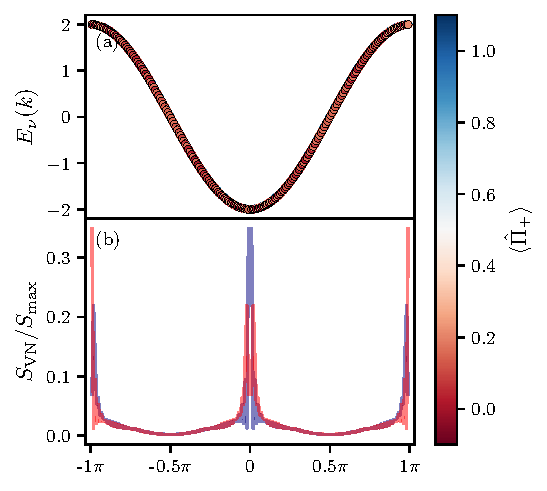
\includegraphics[width=0.45\linewidth]{Figures/band_struct_app_0.001.pdf}
    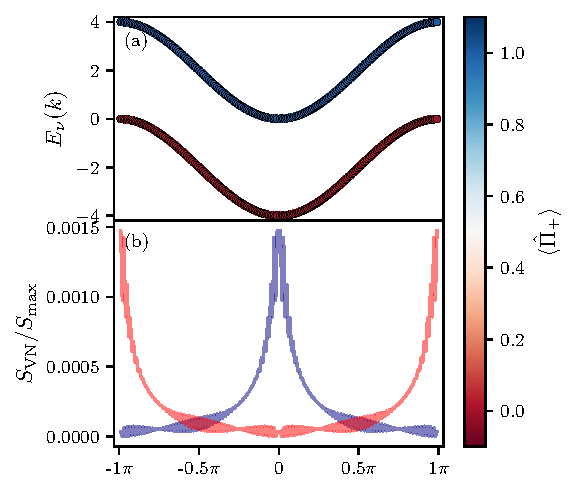
\includegraphics[width=0.45\linewidth]{Figures/band_struct_app_2.000.pdf}
    \caption{(a) ED band structure and entanglement for (a) a slow qubit with \mbox{$\Omega = 0.001t$} and (b) a FLoquet qubit \mbox{$\Omega = 2.0t$}. The coloring follows the same convention as Fig.~\ref{fig:fig2}, according to the projection onto the symmetric band of their respective eigenvectors, with blue being symmetric and red anti-symmetric.}\label{fig:app_band_structure}
\end{figure}

Having calculated the numerator, it is useful to separate Eq.~\eqref{eq:app_first_order1} into three terms that show when the expansion is degenerate: The first term corresponds to \mbox{$\mu \neq \nu, p=k$}, the second \mbox{$\mu = \nu, p\neq k$} and the third \mbox{$\mu \neq \nu, p\neq k$}. This results in the following form
\begin{equation}
     \ket{\Phi_\nu^{(1)} (k)} = \frac{g}{2(N+1)} \frac{\xi(k,k)}{2\epsilon_\nu} \ket{k} \otimes \ket{\bar{\nu}}
    +\frac{g}{2(N+1)} \sum_{p \neq k} \ket{p} \otimes \left\{\frac{\xi(k,p)}{-2t(\cos ak - \cos ap)} \ket{\nu} + \frac{\xi(k,p)}{2\epsilon_\nu - 2t(\cos ak - \cos ap)} \ket{\bar{\nu}} \right\}  \label{eq:app_first_order2},
\end{equation}
corresponding to Eq.~\eqref{eq:app_first_order1} in the main text, where the bar notation over $\nu$ explicitly indicates the opposite qubit eigenstate. As discussed in the main text, this is a quantitative approximation describing the selection rules for the different scattering channels which lead to non-trivial superposition of qubit and QPC states that make entanglement possible by mixing the symmetric and antisymmetric bands. 

Let us start with the first term, which becomes dominant in the slow qubit regime as \mbox{$\Omega < \text{min}\abs{\Delta E (k,p)}$}. We project the full hamiltonian Eq.~\eqref{eq:qpc_dd_H} onto the single-$k$ subspace representing the first term by applying \mbox{$\hat{\Pi}_k = \ket{k}\bra{k}\otimes \left(\ket{+}\bra{+}+\ket{-}\bra{-}\right)$} resulting in
\begin{align}
    \hat{\Pi}_k \hat{H} \hat{\Pi}_k^{\dagger} = E(k) \ket{k}\bra{k} + \hat{h}_k,
\end{align}
where the first term acts on the QPC mode labelled by $k$ with \mbox{$E(k) = - 2t \cos(ak)$} and the second term 
\begin{align}
    \hat{h}_k = - \Omega \left(\ket{0}\bra{0}+\ket{1}\bra{1}\right) + \frac{g \xi(k,k) }{N+1}\ket{1}\bra{1}
\end{align}
acts only on the qubit's Hilbert space.

Since the first terms is already diagonal, one only needs to diagonalize \mbox{$\hat{h}_k$}. Its eigenstates
\begin{align}
    \lambda_\pm = \frac{V_k}{2} \mp \Lambda_k
\end{align}
where mbox{$V_k = g\xi(k,k)/(N+1)$} and \mbox{$\Lambda_k = \sqrt{\Omega^2 + V_k^2/4}$}. The corresponding eigenstates are 
\begin{align}
    \ket{\chi_k} = \cos{\beta_k}\ket{+} + \sin{\beta_k}\ket{-}, \quad \ket{\bar{\chi}_k} = -\sin{\beta_k}\ket{+} + \cos{\beta_k}\ket{-}
\end{align}
in terms of the mixing angle \mbox{$\tan{2\beta_k} = V_k/(2\Omega)$}. 

Then, any vector belonging to the subspace onto which \mbox{$\hat{\Pi}_k$} projects is a superposition of the form
\begin{align}
    \ket{v} = \ket{k} \otimes \left(\alpha \ket{\chi_k} + \beta \ket{\bar{\chi}_k}\right),
\end{align}
therefore all are in a superposition of symmetric and antisymmetric states, with maximum mixing as $\Omega\rightarrow 0$. However, this fact does not translate to entanglement between the QPC and the qubit. In fact, to first order in $g$, the eigenstates in the subspace of \mbox{$\hat{\Pi}_k$} are always a product state, despite the fact that they mix between qubit eigenstates, since they only involve a single QPC $k$ state. Therefore, any entanglement between detector and system in the slow-qubit regime is only due to higher order correction in $g$.

This same analysis applies to the second term which dominates near the maxima and minima of the Brillouin zone. Although, it involves two distinct QPC $k$-states, it does not mix between qubit eigenstates and the eigenstates pf its relevant subspace will always be in a product state between the QPC and the qubit. Thus, the second term does not contribute to entanglement to first order in $g$ either.

The third term is the only one that simultaneously mixes between qubit eigenstates and distinct QPC $k$-states. It is the only one that contributes to entanglement at first order in $g$ when it dominates. As discussed in the main text, this happens when the resonance condition Eq.~\eqref{eq:resonance_condition} is satisfied. This is the reason behind the large entanglement entropy for the resonant band in [II] depicted in Fig.~\ref{fig:fig2}(b)-(c).

%The first term is degenerate when \mbox{$\epsilon_\nu=\pm \Omega\rightarrow0$} and involves $\ket{\bar{\nu}}$, therefore it does mix between two different bands but only for slow qubits. For a Hamiltonian in which this term dominates, the entanglement of the eigenstates is compared with the hybridization at each eigenenergy in Fig.~\ref{fig:app_band_structure}(a). The states remain weakly hybridized throughout the spectrum, except for pronounced fluctuations near the maxima and minima of the Brillouin zone. This term dominates in regime [I] as discussed in Section \ref{sect:entanglement}.

%On the other hand, the second term is degenerate only in at the edges of the Brillouin zone \mbox{$a k\approx \pm \pi$} but it does not mix between bands, hence it does not contribute to entanglement. This degeneracy is typical for tight-binding Hamiltonians and corresponds to elastic scattering between QPC states. An example of the entanglement and hybridization for a system in which this term dominates is shown in Fig.~\ref{fig:app_band_structure}(b). Here, it is clear that both bands are fully symmetric or antisymmetric and the resulting entanglement entropy of the eigenstates is negligible.

%Finally, the third term does mix between bands and becomes degenerate, depending on the whenever the difference in the energy of \mbox{$k$} modes \mbox{$\Delta E (k,p)$} is equal to the band-gap \mbox{$2\epsilon_\nu$}. Since, we consider a finite lattice, \mbox{$\Delta E (k,p)$} is finite, hence a small enough $2 \epsilon_\nu$ (slow qubit) can avoid this degeneracy. Furthermore, a large enough band gap (fast qubit) will always be larger than \mbox{$\Delta E (k,p)$} due the cosine form of the tight-binding energy. These conditions bound the degenerate region as indicated in Eq.~\eqref{eq:entropy_bounds} and dominates the coherent regime [II] as discussed in \ref{sect:entanglement}. This third term can be interpreted in terms of inelastic scattering, where the QPC exchanges momentum energy with the qubit's own eigenenergy .

%As mentioned in the main text, the gaussian weights select which of the eigenstates dominate at any given point which gives and interpretation of the eigenstate peaks at the minima/maxima of the Brillouin zone in Fig~\ref{fig:app_band_structure}. The semi-classical approximation of the gaussian wavepacket, necessitate that the weights are sharply peaked around the central wavenumber $k_0$, with a group velocity $v_g = 2 t \sin{(ak_0)}$. The weights then select the largest contribution to the state to be the one with $k \approx k_0$, which in turn can be assigned a group velocity $v_g$. Therefore, the entropy peaks seen in Fig~\ref{fig:app_band_structure} corresponds with $v_g \approx 0$. Following the analysis in Section \ref{sect:backaction}, these states have an ill-defined measurement time window and the QPC and qubit remain coupled. 

\twocolumngrid

\end{document}

